%!TEX program = xelatex

\documentclass[11pt,titlepage]{report}
%!TEX root = main.tex

\usepackage[T1]{fontenc}
\usepackage{lmodern}
\usepackage[svgnames]{xcolor}
\usepackage{fontspec} % XeLaTeX required!
\usepackage{graphicx}
\usepackage{circuitikz}
\usepackage{tikz}
\usepackage{pifont}
\usepackage[some]{background}
\usepackage{xltxtra} 
\usepackage{setspace}
\usepackage[absolute]{textpos}
\usepackage[latin1]{inputenc}
\usepackage[english]{babel}
\usepackage{graphicx}
\usepackage{wrapfig}
\usepackage{fullpage}
\usepackage[margin=1in]{geometry}
\usepackage{float}
\usepackage{url}
\usepackage{multicol}
\usepackage{hyperref}
\usepackage{titlepic}
\usepackage{standalone}
\usepackage{siunitx}
\usepackage{booktabs}
\usepackage{amsmath}
\usepackage{unicode-math}
\usepackage{verbatim}
\usepackage{enumitem}
\usepackage{listings}
\usepackage{multirow}
\usepackage{pgfplots}
\pgfplotsset{compat=1.8}
\usepackage{caption} 
\usepackage[parfill]{parskip}
\usepackage{import}
\usepackage[backend=bibtexu,texencoding=utf8,bibencoding=utf8,style=ieee,sortlocale=en_GB,language=auto]{biblatex}
\usepackage[strict,autostyle]{csquotes}
\usepackage[final]{pdfpages}
\usepackage{subcaption}
\usepackage{ifplatform}
%\captionsetup[table]{skip=10pt}


% Fix for includepdf bug in Mac OS X
\newcommand{\insertpdfpath}[1]{
	\ifwindows
	\newcommand{\insertpdf}[2]{\includepdf[pages=##1]{##2}}
	\else
	\newcommand{\insertpdf}[2]{\includepdf[pages=##1]{#1/##2}}
	\fi
}

%set fonts
\setmainfont[Ligatures=TeX]{Myriad Pro}
\setmathfont{Asana Math}
\setmonofont{Lucida Console}

\usepackage{titlesec, color}
\renewcommand{\familydefault}{\sfdefault} %set font family
\renewcommand{\arraystretch}{1.2} %set table vertical spacing
\setlength\parindent{0pt} %no paragraph indent
\hypersetup{ %setup hyperlinks
    colorlinks,
    citecolor=black,
    filecolor=black,
    linkcolor=black,
    urlcolor=black
}

%redesign chapter headings
\definecolor{gray75}{gray}{0.75}
\newcommand{\chapternumber}{\thechapter}
\newcommand{\hsp}{\hspace{20pt}}
\titleformat{\chapter}[hang]{\Huge\bfseries}{\chapternumber\hsp\textcolor{gray75}{|}\hsp}{0pt}{\Huge\bfseries}

%Redefine appendix headers
\renewcommand{\appendixname}{Appendix}
\renewcommand{\appendixtocname}{Appendices}
\renewcommand{\appendixpagename}{Appendices}

%For code listings
\definecolor{black}{rgb}{0,0,0}
\definecolor{browntags}{rgb}{0.65,0.1,0.1}
\definecolor{bluestrings}{rgb}{0,0,1}
\definecolor{graycomments}{rgb}{0.4,0.4,0.4}
\definecolor{redkeywords}{rgb}{1,0,0}
\definecolor{bluekeywords}{rgb}{0.13,0.13,0.8}
\definecolor{greencomments}{rgb}{0,0.5,0}
\definecolor{redstrings}{rgb}{0.9,0,0}
\definecolor{purpleidentifiers}{rgb}{0.01,0,0.01}


\lstdefinestyle{csharp}{
language=[Sharp]C,
showspaces=false,
showtabs=false,
breaklines=true,
showstringspaces=false,
breakatwhitespace=true,
escapeinside={(*@}{@*)},
columns=fullflexible,
commentstyle=\color{greencomments},
keywordstyle=\color{bluekeywords}\bfseries,
stringstyle=\color{redstrings},
identifierstyle=\color{purpleidentifiers},
basicstyle=\ttfamily\small}

\lstdefinestyle{c}{
language=C,
showspaces=false,
showtabs=false,
breaklines=true,
showstringspaces=false,
breakatwhitespace=true,
escapeinside={(*@}{@*)},
columns=fullflexible,
commentstyle=\color{greencomments},
keywordstyle=\color{bluekeywords}\bfseries,
stringstyle=\color{redstrings},
identifierstyle=\color{purpleidentifiers},
}

\lstdefinestyle{matlab}{
language=Matlab,
showspaces=false,
showtabs=false,
breaklines=true,
showstringspaces=false,
breakatwhitespace=true,
escapeinside={(*@}{@*)},
columns=fullflexible,
commentstyle=\color{greencomments},
keywordstyle=\color{bluekeywords}\bfseries,
stringstyle=\color{redstrings},
identifierstyle=\color{purpleidentifiers}
}

\lstdefinestyle{vhdl}{
language=VHDL,
showspaces=false,
showtabs=false,
breaklines=true,
showstringspaces=false,
breakatwhitespace=true,
escapeinside={(*@}{@*)},
columns=fullflexible,
commentstyle=\color{greencomments},
keywordstyle=\color{bluekeywords}\bfseries,
stringstyle=\color{redstrings},
identifierstyle=\color{purpleidentifiers}
}

\lstdefinestyle{xaml}{
language=XML,
showspaces=false,
showtabs=false,
breaklines=true,
showstringspaces=false,
breakatwhitespace=true,
escapeinside={(*@}{@*)},
columns=fullflexible,
commentstyle=\color{greencomments},
keywordstyle=\color{redkeywords},
stringstyle=\color{bluestrings},
tagstyle=\color{browntags},
morestring=[b]",
  morecomment=[s]{<?}{?>},
  morekeywords={xmlns,version,typex:AsyncRecords,x:Arguments,x:Boolean,x:Byte,x:Char,x:Class,x:ClassAttributes,x:ClassModifier,x:Code,x:ConnectionId,x:Decimal,x:Double,x:FactoryMethod,x:FieldModifier,x:Int16,x:Int32,x:Int64,x:Key,x:Members,x:Name,x:Object,x:Property,x:Shared,x:Single,x:String,x:Subclass,x:SynchronousMode,x:TimeSpan,x:TypeArguments,x:Uid,x:Uri,x:XData,Grid.Column,Grid.ColumnSpan,Click,ClipToBounds,Content,DropDownOpened,FontSize,Foreground,Header,Height,HorizontalAlignment,HorizontalContentAlignment,IsCancel,IsDefault,IsEnabled,IsSelected,Margin,MinHeight,MinWidth,Padding,SnapsToDevicePixels,Target,TextWrapping,Title,VerticalAlignment,VerticalContentAlignment,Width,WindowStartupLocation,Binding,Mode,OneWay,xmlns:x}
}

\lstdefinestyle{matlab}{
language=Matlab,
showspaces=false,
showtabs=false,
breaklines=true,
showstringspaces=false,
breakatwhitespace=true,
escapeinside={(*@}{@*)},
columns=fullflexible,
commentstyle=\color{greencomments},
keywordstyle=\color{bluekeywords}\bfseries,
stringstyle=\color{purpleidentifiers},
identifierstyle=\color{purpleidentifiers}
}

%defaults
\lstset{
basicstyle=\ttfamily\small,
extendedchars=false,
numbers=left,
numberstyle=\ttfamily\tiny,
stepnumber=1,
tabsize=4,
numbersep=5pt
}
\addbibresource{../../library/bibliography.bib}

\let\vec\vecold
\newcommand{\vec}[1]{\mathbf{#1}}


\definecolor{myblue}{RGB}{91,155,213}

\usetikzlibrary{shapes,arrows}
\tikzstyle{rectangle} = [
	rectangle,
	draw=myblue,
	fill=myblue,
	text=white,
    text width=8em, 
    text centered,
    rounded corners,
    minimum height=6em
]
\tikzstyle{rectangle} = [
	draw=myblue,
	fill=myblue,
	text=white,
    text width=8em, 
    text centered,
    minimum height=6em
]

\tikzstyle{line} = [
	draw=myblue,
	text=myblue,
	myblue,
	>=triangle 90
]

% Opbouw:
% - Inleiding: weten afstand, gewenste afstand, hoek, gewenste hoek, hoe PWM waardes bepalen zodat bereikt wordt
% reductie dimensionaliteit, twee onafhankelijk werkende systemen
% - Controllers:
% * Distance controller
% * Angle controller
% - Excitation mapping
% - Solving the models
\begin{document}

\chapter{Controller}
\label{ch:control}
\section{Introduction}
At this point we assume certain things to be known; the current distance to the next waypoint, KITT's current angle and KITT's ideal angle. A system must be designed which controls KITT in a way that the distance to the next waypoint reduces to zero. In other words, KITT needs to be controlled to the next waypoint.

To achieve this seemingly easy task, we invented a method which we call \textit{reduction of dimensionality}. Controlling KITT to a given position can be seen as a two-dimensional problem. Consider KITT a black box, then the inputs are given by the driving and steering excitation, and the output by the current position. One could create a model of the whole system. However, this model would be non-linear and therefore hard to handle. A better approach seemed to divide the complex two-dimensional problem into two less complicated one-dimensional problems; \textbf{(1)}, controlling KITT's angle in a way that KITT drives a specified trajectory and \textbf{(2)}, controller KITT's speed in a way that KITT stops at the specified target. This concept is shown in Figure~\ref{fig:ctrl-reduction}.

\begin{figure}
	\centering
	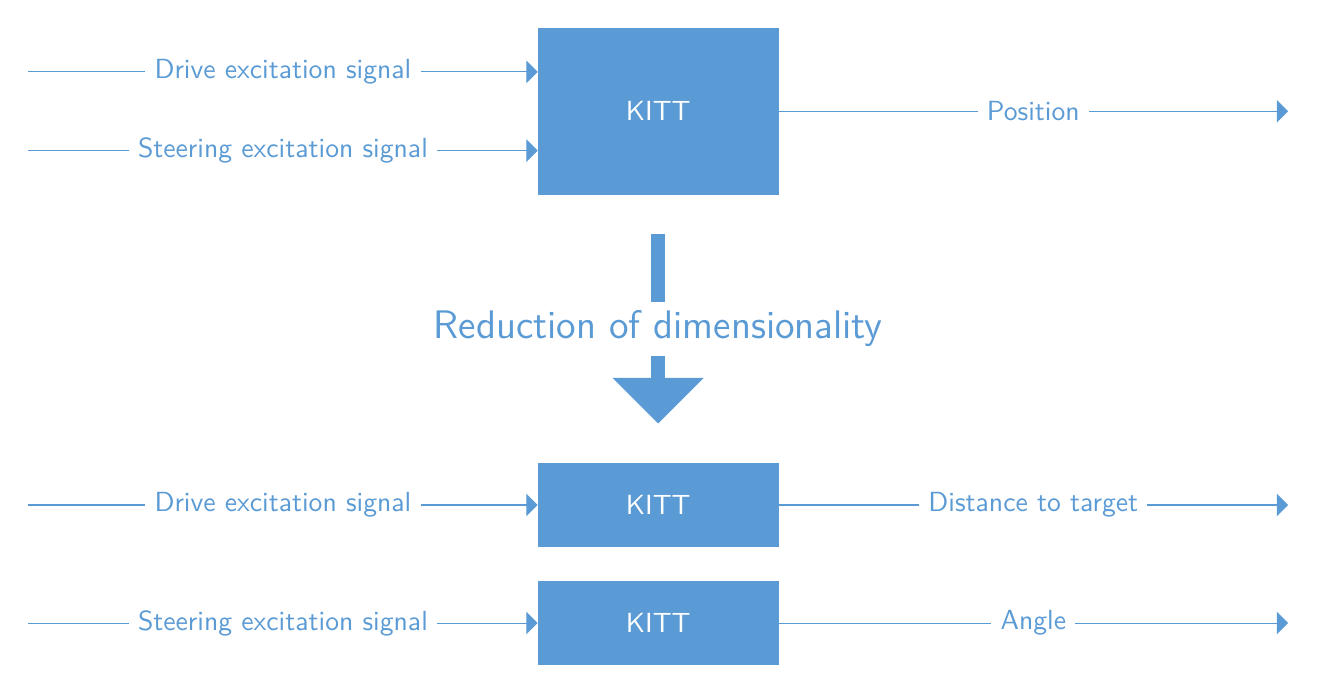
\begin{tikzpicture}[node distance=5cm, auto]
		% Nodes
		\node [rectangle] (kitt) {KITT} (0,0);

		% Input edges
		\path [line, ->, yshift=0.5cm] (-8,0) -- node [anchor=center,fill=white] {Drive excitation signal} ([yshift=0.5cm]kitt.west);
		\path [line, ->, yshift=-0.5cm] (-8,0) -- node [anchor=center,fill=white] {Steering excitation signal} ([yshift=-0.5cm]kitt.west);

		% Output edges
		\path [line, ->] (kitt.east) -- node [anchor=center,fill=white] {Position} (8,0);

		% Bottom thing 1
		\begin{scope}[yshift=-5cm]
			% Nodes
			\node [rectangle, minimum height=3em] (kitt2) {KITT} (0,0);

			% Input edges
			\path [line, ->] (-8,0) -- node [anchor=center,fill=white] {Drive excitation signal} (kitt2.west);

			% Output edges
			\path [line, ->] (kitt2.east) -- node [anchor=center,fill=white] {Distance to target} (8,0);
		\end{scope}

		% Bottom thing 1
		\begin{scope}[yshift=-6.5cm]
			% Nodes
			\node [rectangle, minimum height=3em] (kitt3) {KITT} (0,0);

			% Input edges
			\path [line, ->] (-8,0) -- node [anchor=center,fill=white] {Steering excitation signal} (kitt3.west);

			% Output edges
			\path [line, ->] (kitt3.east) -- node [anchor=center,fill=white] {Angle} (8,0);
		\end{scope}
		
		% Connection
		\path [line, ->, line width=5pt,] ([yshift=-0.5cm]kitt.south) -- node [anchor=center,fill=white] {\Large Reduction of dimensionality} ([yshift=0.5cm]kitt2.north);
	\end{tikzpicture}
	\caption{Reduction of dimensionality}
	\label{fig:ctrl-reduction}
\end{figure}


% One of the two mid-term challenges was for KITT to drive autonomously at a wall and stop as close as possible in front of that wall. We designed a controller to accomplish this seemingly easy task. The controller consists of two components; the \textit{observer} and the \textit{compensator}. We will explain both of these in further detail.

\section{Observer design}
The controller must have knowledge of the current position and velocity of the car to be able to successfully control KITT. Generalizing, we can say that the controller must have knowledge of the current \textit{state} of KITT. The observer's task is to keep track of the internal state of KITT. This internal state consists of a linear combination of all generalized positions and momenta of respectively all inductive and capacitive components of the system. If we consider KITT a state-space model, we can define inputs and an output. Figure~\ref{fig:ctrl-model} shows this line of thought.

\begin{figure}
	\centering
	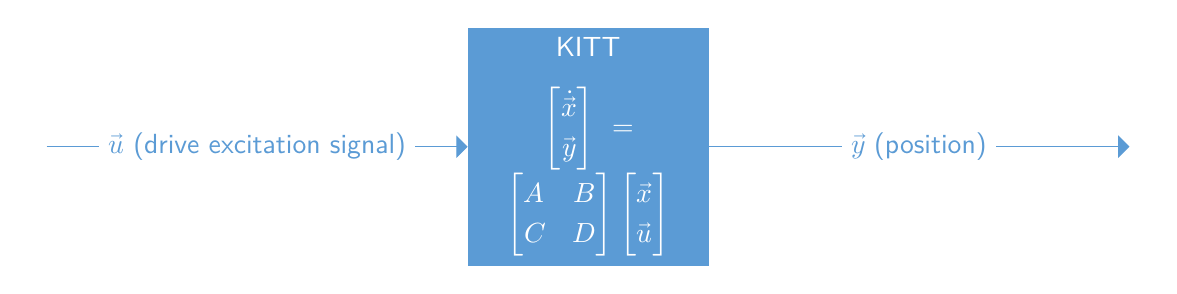
\begin{tikzpicture}[node distance = 7cm, auto]
		% Nodes
		\node [] (input) {};
		\node [rectangle, right of=input] (kitt) {KITT \\[1em] $\begin{bmatrix} \dot{\vec{x}} \\ \vec{y} \end{bmatrix} = \begin{bmatrix} \mat{A} & \mat{B} \\ \mat{C} & \mat{D} \end{bmatrix} \begin{bmatrix} \vec{x} \\ \vec{u} \end{bmatrix}$};
		\node [right of=kitt] (output) {};
		% Edges
		\path [line, ->] (input) -- node [anchor=center,fill=white] {$\vec{u}$ (drive excitation signal)} (kitt);
		\path [line, ->] (kitt) -- node [anchor=center,fill=white] {$\vec{y}$ (position)} (output);
	\end{tikzpicture}
	\caption{State-space based model of KITT}
	\label{fig:ctrl-model}
\end{figure}

The observer observes the input $\vec{u}$ and output $\vec{y}$ and determines, by doing that, the internal state $\vec{x}$ of KITT. We modeled the observer by making also use of a state-space representation. Logically thinking, the observer must obey to two constraints; \textbf{(1)}, the internal state $\hat{\vec{x}}$ of the observer must converge to $\vec{x}$ if $t \to \infty$ and \textbf{(2)}, if $\hat{\vec{x}} = \vec{x}$, then the states should not diverge. To fulfill \textbf{(1)}, we introduce a feedback matrix $\mat{L}$ which will be discussed later, and to satisfy \textbf{(2)}, the system, input-, output- and feed-through matrix of the observer should match KITT's.

\begin{figure}[H]
	\centering
	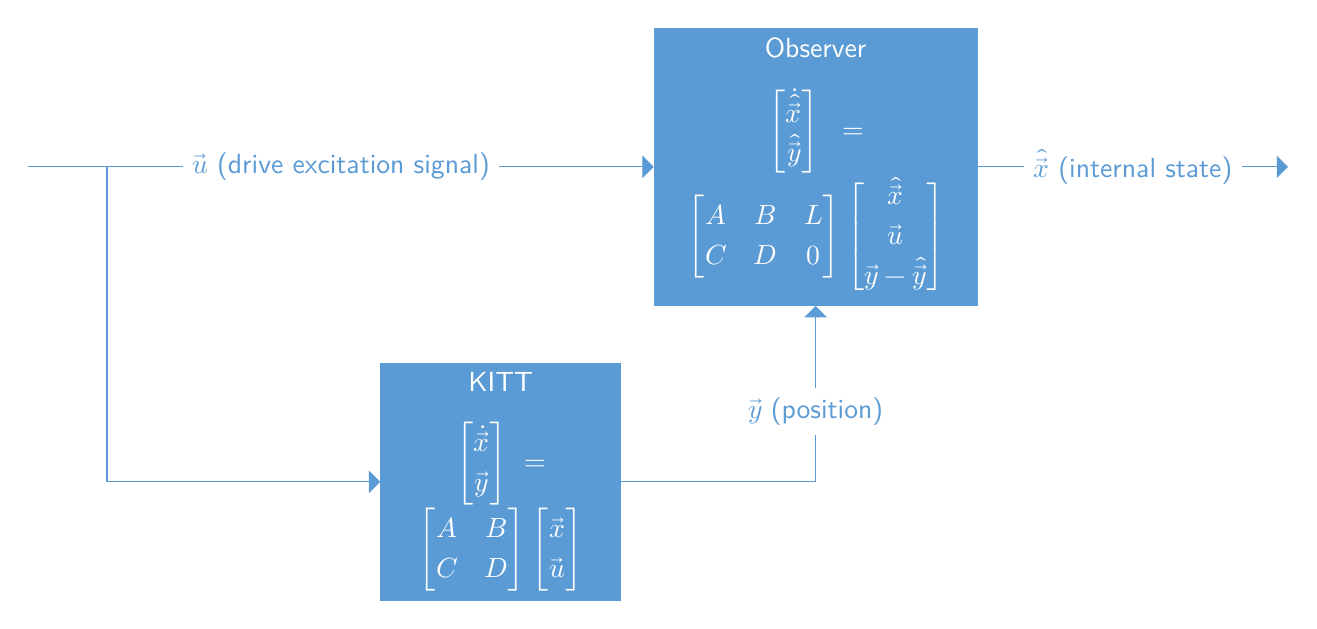
\begin{tikzpicture}[node distance = 6.5cm, auto]
		% Nodes
		\node [rectangle] (kitt) at (6,0) {KITT \\[1em] $\begin{bmatrix} \dot{\vec{x}} \\ \vec{y} \end{bmatrix} = \begin{bmatrix} \mat{A} & \mat{B} \\ \mat{C} & \mat{D} \end{bmatrix} \begin{bmatrix} \vec{x} \\ \vec{u} \end{bmatrix}$};
		\node [rectangle, text width=11em] (observer) at (10,4) {Observer \\[1em] $\begin{bmatrix} \dot{\hat{\vec{x}}} \\ \hat{\vec{y}} \end{bmatrix} = \begin{bmatrix} \mat{A} & \mat{B} & \mat{L} \\ \mat{C} & \mat{D} & 0 \end{bmatrix} \begin{bmatrix} \hat{\vec{x}} \\ \vec{u} \\ \vec{y} - \hat{\vec{y}} \end{bmatrix}$};

		% Coordinates
		\coordinate (input) at (0,4);
		\coordinate (input_split) at (1,4);
		\coordinate (output) at (16,4);

		% Edges
		\path [line, ->] (input) -- node [anchor=center,fill=white] {$\vec{u}$ (drive excitation signal)} (observer.west);
		% \path (input) edge [->, pos=0.3] node {$\vec{u}$ (drive excitation signal)} (observer.west);
		\path [line, ->] (kitt.east) -| node [anchor=center,fill=white,pos=0.7] {$\vec{y}$ (position)} (observer.south);
		\path [line, ->] (input_split) |- node [] {} (kitt.west);
		\path [line, ->] (observer.east) -- node [anchor=center,fill=white] {$\hat{\vec{x}}$ (internal state)} (output);
	\end{tikzpicture}
	\caption{State-space based model of KITT and the observer}
	\label{fig:ctrl-model-observer}
\end{figure}

We can show constraint \textbf{(1)} by evaluating the error $\vec{e}=\vec{x}-\hat{\vec{x}}$.

\begin{equation} \label{eq:ctrl-err}
	\dot{\vec{e}}=\dot{\vec{x}} - \dot{\hat{\vec{x}}} = \mat{A} (\vec{x} - \hat{\vec{x}}) - \mat{L} (\vec{y} - \hat{\vec{y}}) = (\mat{A} - \mat{L} \mat{C}) (\vec{x} - \hat{\vec{x}}) = (\mat{A} - \mat{L}\mat{C}) \vec{e}
\end{equation}

Equation~\ref{eq:ctrl-err} tells us the the system is observable, if $\mat{A} - \mat{L}\mat{C}$ renders $\vec{e}$ asymptotically stable. This defines the observability of the pair $(\mat{C}, \mat{A})$. The duality between observability and controllability tells us that $(\mat{C},\mat{A})$ is observable if $(\tr{\mat{A}},\tr{\mat{C}})$ is controllable. Therefore, we used the MATLAB command \texttt{place(A',C',poles)'} to calculate $\mat{L}$.

\begin{figure}[H]
	\centering
	\begin{tikzpicture}[node distance=2cm]
		\bgComponentNoBond{bat}{$S_e:v$}
		\bgComponent{}{1-1}{1}{right of=}{bat}{inbond}
		\bgComponent{}{ind}{$I:L$}{above of=}{1-1}{inbond}
		\bgComponent{}{res1}{$R:R$}{below of=}{1-1}{inbond}

		\bgComponentWithBondLabel{}{gy}{GY}{right of=}{1-1}{inbond}{}{$e_1=e$}{$f_1=i$}

		\bgComponentWithBondLabel{node distance=3cm}{loss}{TF}{right of=}{gy}{inbond}{}{$k_t f_1=\tau_m$}{$k_t^{-1} e_1=\omega_m$}
		\bgComponentWithBondLabel{node distance=3cm}{conv}{TF}{right of=}{loss}{inbond}{}{$k_g \tau_m=\tau_w$}{$k_g^{-1} \omega_m = \omega_w$}
		\bgComponentWithBondLabel{node distance=3cm}{1-2}{1}{right of=}{conv}{inbond}{}{$r_w^{-1} \tau_w=F$}{$r_w \omega_w=v$}


		\bgComponent{}{mass}{$I:m$}{above of=}{1-2}{inbond}
		\bgComponent{}{res2}{$R:\rho$}{right of=}{1-2}{inbond}
	\end{tikzpicture}
	\caption{Bond graph representation of KITT's model}
	\label{fig:ctrl-bond}
\end{figure}

The only thing which remained was determining the system matrices $\mat{A}$, $\mat{B}$, $\mat{C}$ and $\mat{D}$ and  the feedback matrix $\mat{L}$. For the system matrices, we did two things; \textbf{(1)}, we used the \textit{System Identification Toolbox} of MATLAB in combination with experiments to fit a state-space model, and \textbf{(2)}, we used the bond graph depicted in Figure~\ref{fig:ctrl-bond} to derive the state-space model shown in Equation~\ref{eq:ctrl-bond-model}. Here the battery voltage is denoted by $v$, the inductance of the motor by $L$, the internal resistance of the motor by $R$, the motor constant by $k_t$, the gear constant by $k_g$, the radius of the wheels by $r_w$, the mass of KITT by $m$, the rolling resistance coefficient by $\rho$ and $k_t k_g/r_w$ by $r$ and a generalized notation of position and velocity is used. The observability matrix $\mathcal{O}$ and the controllability matrix $\mathcal{C}$ revealed that the system was both observable and controllable. Eventually we let $L \to 0$ to reduce the order of the model to two.

\begin{align} \label{eq:ctrl-bond-model}
	\dot{\vec{x}} = \frac{d}{dt}
	\begin{bmatrix}
		q_m \\
		f_m \\
		f_L
	\end{bmatrix} &= \mat{A} \vec{x} + \mat{B} \vec{u} =
	\begin{bmatrix}
		0 & 1 & 0 \\
		0 & -\frac{\rho}{m} & \frac{r}{m} \\
		0 & -\frac{r}{L} & -\frac{R}{L}
	\end{bmatrix}
	\begin{bmatrix}
		q_m \\
		f_m \\
		f_L
	\end{bmatrix} +
	\begin{bmatrix}
		0 \\
		0 \\
		\frac{1}{L}
	\end{bmatrix} v \\
	\vec{y} = q_m &= \mat{C} \vec{x} + \mat{D} \vec{u} =
	\begin{bmatrix}
		1 & 0 & 0
	\end{bmatrix}
	\begin{bmatrix}
		q_m \\
		f_m \\
		f_L
	\end{bmatrix}
\end{align}

To determine the poles, we defined a measure of performance for each pair of poles. We let the observer track measurement data which consisted of the drive excitation $\vec{u}$ and distances measured $\vec{y}$. The observer produced the tracked distance $\mat{C} \hat{\vec{x}} = \hat{\vec{y}}$. If the time interval between $\vec{y}_n$ and $\vec{y}_{n+1}$ is $T$, then we defined the error $e_i$ of experiment $i$ to be

\begin{equation}
	e_i = \int_{0}^{t_f} || \vec{y}(t) - \hat{\vec{y}}(t) || dt = \sum_{0}^{N} ||\vec{y}_n - \hat{\vec{y}_n} ||.
\end{equation}

Figure~\ref{fig:ctrl-poles} shows the error of many different pairs of poles. It is clear that there exists a maximum where $\lambda_1=\lambda_2$. This is obvious, because using Jordan's normal form, one can show that when $\lambda_1 = \lambda_2$, the response is critically damped. Also, $\lambda_1 = \lambda_2$ renders the system matrix non-diagonalizable, which explains the presence of the white line at every point where $\lambda_1=\lambda_2$. At last, the reason the maximum is not located at $(-\infty,-\infty)$, which corresponds with the highest convergence of the observer possible, is because we are also dealing with latency, meaning that $t_{n+1}-t_n>0$.  

\section{Compensator design}
Lets go back to Figure~\ref{fig:ctrl-model} and say we actually know the internal state $\vec{x}$. System identification and modeling revealed that when $\vec{x}$ is of the form $\tr{(d,\dot{d})}$, where $d$ is the distance measured and $\dot{d}$ the velocity of KITT, $\mat{A}$, $\mat{B}$, $\mat{C}$ and $\mat{D}$ are of the form

\begin{equation}
	\mat{A} = \begin{bmatrix}
		0 & a_1 \\
		0 & a_2
	\end{bmatrix}, \mat{B} = \begin{bmatrix}
		0 \\
		b
	\end{bmatrix}, \mat{C} = \begin{bmatrix}
		1 & 0
	\end{bmatrix}, \mat{D} = 0.
\end{equation}

Let us introduce the feedback law $\vec{u} = -\mat{K}(\vec{x}-\vec{x}_{ref})$. Rewriting the state-space model equations yields

\begin{equation} \label{eq:ctrl-comp}
	\dot{\vec{x}} = (\mat{A} - \mat{B} \mat{K}) \vec{x} + \mat{B} \mat{K} \vec{x}_{ref}.
\end{equation}


Here $x_{ref}=\tr{(d_{ref},0)}$. If we argue that $\mat{A} - \mat{B} \mat{K}$ renders the system asymptotically stable, then rewriting Equation~\ref{eq:ctrl-comp} using $\dot{\vec{x}} \to 0$ when $t \to \infty$ yields

\begin{equation} \label{eq:ctrl-comp-feedback}
	(\mat{B} \mat{K} - \mat{A}) \vec{x} = \mat{B} \mat{K} \vec{x}_{ref} = 
	\left( \begin{bmatrix}
		0 \\
		b
	\end{bmatrix} \begin{bmatrix}
		k_1 & k_2
	\end{bmatrix} - \begin{bmatrix}
		0 & a_1 \\
		0 & a_2
	\end{bmatrix} \right) \begin{bmatrix}
		x_1 \\
		x_2
	\end{bmatrix} = \begin{bmatrix}
		0 \\
		b
	\end{bmatrix} \begin{bmatrix}
		k_1 & k_2
	\end{bmatrix} \begin{bmatrix}
		d_{ref} \\
		0
	\end{bmatrix}.
\end{equation}

Further simplifying Equation~\ref{eq:ctrl-comp-feedback} yields

\begin{equation} \label{eq:ctrl-comp-feedback2}
	\begin{bmatrix}
		 -x_2 a_1 \\
		x_1 b k_1 + x_2 (b k_2 - a_2)
	\end{bmatrix} = \begin{bmatrix}
		0 \\
		d_{ref} b k_1
	\end{bmatrix}.
\end{equation}

Evaluating Equation~\ref{eq:ctrl-comp-feedback2} yields $x_1$ = $d_{ref}$ and $x_2=0$. This means that the model shown in Figure~\ref{fig:ctrl-model} converges to a state where KITT is not moving at a specified distance $d_{ref}$. In other words, we specify the position at which KITT stops moving. The only thing which remains, is determining the poles of $\mat{A} - \mat{B} \mat{K}$. We want KITT to stop at our specified position as fast as possible, without overshooting. Therefore, KITT must critically damped converge to a distance $d_{ref}$. If $\lambda_1$ and $\lambda_2$ are the eigenvalues of $\mat{A} - \mat{B} \mat{K}$, then $\lambda_1$ and $\lambda_2$ must be real and negative with $\lambda_1 - \lambda_2$ minimized. The exact value of $\lambda_1$ and $\lambda_2$ depends on the latency we are dealing with. We adjusted these eigenvalues on-the-go to achieve an optimized result.

\section{Controller design}
Putting together the observer and the compensator together yields the controller. This closed-loop system is depicted in Figure~\ref{fig:ctrl-controller}. Note that we discussed the design of the observer and compensator, as if they could be designed separately. This is exactly what the separation principle states. 

\begin{figure}[H]
	\centering
	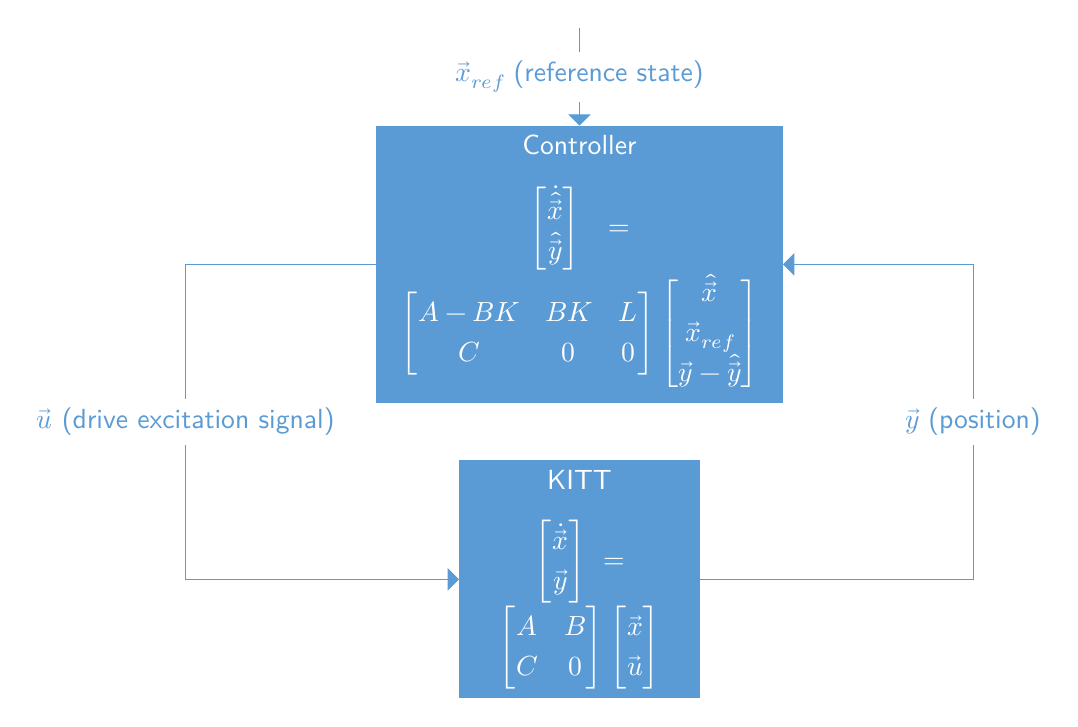
\begin{tikzpicture}[node distance = 6.5cm, auto]
		% Nodes
		\node [rectangle] (kitt) at (0,0) {KITT \\[1em] $\begin{bmatrix} \dot{\vec{x}} \\ \vec{y} \end{bmatrix} = \begin{bmatrix} \mat{A} & \mat{B} \\ \mat{C} & 0 \end{bmatrix} \begin{bmatrix} \vec{x} \\ \vec{u} \end{bmatrix}$};
		\node [rectangle, text width=14em] (controller) at (0,4) {Controller \\[1em] $\begin{bmatrix} \dot{\hat{\vec{x}}} \\ \hat{\vec{y}} \end{bmatrix} = \begin{bmatrix} \mat{A}-\mat{B}\mat{K} & \mat{B}\mat{K} & \mat{L} \\ \mat{C} & 0 & 0 \end{bmatrix} \begin{bmatrix} \hat{\vec{x}} \\ \vec{x}_{ref} \\ \vec{y} - \hat{\vec{y}} \end{bmatrix}$};

		% Edges
		\path [line, ->] (controller.west) -| node [anchor=center,fill=white,pos=1] {$\vec{u}$ (drive excitation signal)} (-5,2) |- (kitt.west);
		\path [line, ->] (kitt.east) -| node [anchor=center,fill=white,pos=1] {$\vec{y}$ (position)} (5,2) |- (controller.east);
		\path [line, ->] (0,7) -- node [anchor=center,fill=white] {$\vec{x}_{ref}$ (reference state)} (controller.north);
	\end{tikzpicture}
	\caption{State-space based controller of KITT}
	\label{fig:ctrl-controller}
\end{figure}

\section{Controller implementation}
Now only three undiscussed aspects of the controller remain; correctly receiving the distance measured, converting the drive excitation signal to a PWM signal and solving the state-space model. We will briefly discuss these aspects in the following paragraphs.

The ultrasonic sensors we used, did not always output correct values. We therefore developed a discrete time finite impulse response low-pass filter and a so-called prediction filter to purify our signals. These filters are further discussed in Appendix~\ref{app:signal-filtering}. We also discussed a method to use the Doppler effect to increase measurement accuracy. This method is described in Appendix~\ref{app:doppler}.

After some testing, we noticed that the motors did not do anything with a PWM signal ranging from $145$ to $155$. This motivated us to the following \textit{mapping}.

\begin{equation} \label{eq:ctrl-mapping}
	\text{PWM}(u) = \left\{ \begin{array}{l l}
		155 + a_1 u + a_2 u^3 & \quad \text{ if } u > u_t, \\
		145 + a_1 u + a_2 u^3 & \quad \text{ if } u < -u_t.
	\end{array} \right.
\end{equation}

Here the drive excitation is denoted by $u$, the first-order coefficient (FOC) by $a_1$, the third-order coefficient (TOC) by $a_2$ and the excitation threshold by $u_t$. The FOC mostly determines the relation between the excitation and PWM signal. To tweak for non-linear effects, we introduced the TOC. The combination of the latency and minimum driving speed of KITT determines the accuracy at which we can control KITT. Therefore, we can only correct for certain errors. This is the reason we introduced a excitation threshold; the threshold prevents oscillations due to latency.

Finally, we had to solve the designed state-space model. There are numerous numerical methods which are designed for solving differential equations. To improve the convergence of a numerical approximation, one can use two methods; \textbf{(1)}, use higher-order methods which inherently converge faster, or \textbf{(2)}, instead of evaluating one time step $T$, evaluate $N$ steps with time $T/N$. We used a fourth-order method of the Runge-Kutta family to approximate the state-space model. Appendix~\ref{app:num} gives a brief introduction to numerically solving KITT.

\end{document}